% !TeX encoding = UTF-8
% !TeX spellcheck = de_DE

%% Dies gibt Warnungen aus, sollten veraltete LaTeX-Befehle verwendet werden
\RequirePackage[l2tabu, orthodox]{nag}

\documentclass[utf8,biblatex]{lni}
\bibliography{lni-paper-example-de}

%% Schöne Tabellen mittels \toprule, \midrule, \bottomrule
\usepackage{booktabs}

%% Zu Demonstrationszwecken
\usepackage[math]{blindtext}
\usepackage{mwe}

%% BibLaTeX-Sonderkonfiguration,
%% falls man schnell eine existierende Bibliographie wiederverwenden will, aber nicht die .bib-Datei händisch anpassen möchte.
%% Bitte \iffalse und \fi entfernen, dann ist diese Konfiguration aktiviert.

\iffalse
\AtEveryBibitem{%
  \ifentrytype{article}{%
  }{%
    \clearfield{doi}%
    \clearfield{issn}%
    \clearfield{url}%
    \clearfield{urldate}%
  }%
  \ifentrytype{inproceedings}{%
  }{%
    \clearfield{doi}%
    \clearfield{issn}%
    \clearfield{url}%
    \clearfield{urldate}%
  }%
}
\fi

\begin{document}
%%% Mehrere Autoren werden durch \and voneinander getrennt.
%%% Die Fußnote enthält die Adresse sowie eine E-Mail-Adresse.
%%% Das optionale Argument (sofern angegeben) wird für die Kopfzeile verwendet.
\title[Suchen und Grovers]{Quanten Computing verstehen: Suchen und Grovers Algorithmus}
%%%\subtitle{Untertitel / Subtitle} % falls benötigt
\author[Sabrina Cielas \and Till Pilarczyk]
{Sabrina Cielas\footnote{Hochschule Düsseldorf, Gebäude 4, Münsterstraße 156, 40476 Düsseldorf, Deutschland \email{sabrina.cielas@study.hs-duesseldorf.de}, Matr.: 771074} \and
 Till Pilarczyk\footnote{Hochschule Düsseldorf, Gebäude 4, Münsterstraße 156, 40476 Düsseldorf, Deutschland \email{till.pilarczyk@study.hs-duesseldorf.de}, Matr.: 765335}}
\startpage{1} % Beginn der Seitenzählung für diesen Beitrag
\editor{Hochschule Düsseldorf}    % Namen der Herausgeber
\booktitle{Modul: QCV} % Name des Tagungsband; optional Kurztitel
%\yearofpublication{2017}
%%%\lnidoi{18.18420/provided-by-editor-02} % Falls bekannt
\maketitle %\thispagestyle{}
\thispagestyle{fancy}

\begin{abstract}
Suchprobleme können von Klassischen Computern nicht effizient gelöst werden. Bei einer Suche mit Quantencomputer und dem Grover Algrothmus wird eine Quadratische beschleunigung erreicht werden. Der Grover Algorithmus setzt diese Suche in unstrukturierten Daten perfekt um. Dabei wird in Schritten die Amplitude des gesuchten Elementes gesteigert und alle anderen Amplitiden gesenkt. Der Algrotihmus hat verschiedene Varianten, so kann nach meheren oder unbekannt vielen Lösungen und dem Minum gesucht werden. Die Laufzeit wird dabei nicht schlechter. Mithilfe des Grover Algrotihmus lassen sich jedoch nach aktuellem Stand keine NP Probleme effizient lösen Daher wird der Quantencomputer mithilfe des Algorithmus nicht zu einem Allheilmittel.
\end{abstract}

\begin{keywords}
Quantencomputer \and Quantum Computing \and Grovers-Algorithmen
\end{keywords}

\section{Einleitung $\mathbf{\textsubscript{\small sc}}$}
Viele Berechnungsprobleme sind in ihrer Essenz Suchprobleme: Optimierungsprobleme sind die Suche nach der optimalen Lösung, der Versuch, eine kryptografische Verschlüsselung zu brechen, ist die Suche nach dem korrekten Schlüssel. Um diese Probleme effizient lösen zu können, ergibt sich die große Relevanz der Suchalgorithmen.
\\
Diese Arbeit ist im Rahmen des Moduls “Quantencomputer verstehen - Grundlagen und Anwendungen” an der Hochschule Düsseldorf bei Prof. Dr. Holger Schmidt entstanden. In dem Modul wurden zunächst gemeinsam die Grundlagen des Themengebiets Quantencomputer erarbeitet. Darauf aufbauend wurden durch die Studierenden Seminarvorträge vorbereitet, welche verschiedene Themengebiete tiefer gehend beleuchten und im Kurs vorgestellt wurden. Dies ist die schriftliche Ausarbeitung zu dem Seminarvortrag “Suchen \& Grovers Algorithmus”. Es werden die im Modul erarbeiteten Grundlagen als bekannt vorausgesetzt.
\newline
\\
Diese Seminararbeit fokussiert sich auf den von Dr. Lov Grover entwickelten Quantensuchalgorithmus. Außerdem werden dessen verschiedene Varianten und die möglichen Anwendungsgebiete vorgestellt.
Von zentralem Interesse ist dabei, ob Quantencomputer mit dem Grover-Suchalgorithmus zukünftig jene Probleme effizient lösen können, für die es mit klassischen Computern bisher keine geeigneten Lösungen gibt. 
Aus diesem Grund findet die Laufzeit des Suchalgorithmus besondere Betrachtung, um im Fazit diese Frage angemessen beantworten zu können. 
Als Hauptquelle diente Kapitel 6 “Suchen” aus dem Buch “Quantum Computing verstehen: Grundlagen - Anwendungen - Perspektiven” von Matthias Homeister.
\newline
\\
TODO: Aufbau der Arbeit

\section{Aufgabenstellung $\mathbf{\textsubscript{\small sc}}$}
Das grundlegende Problem, welches im Folgenden betrachtet wird, ist die unstrukturierte Suche. 
Es soll ein gegebenes Datum aus einer Menge von Datensätzen gefunden werden. 
Die Datensätze sind dabei entweder gänzlich unsortiert oder nach einem Kriterium, welches für die Suche keine Relevanz besitzt. 
Die Suche kann mit einer Funktion $\mathbf{f(x)}$ abgebildet werden, welche die Datensätze $\mathbf{x}$ als Eingabe akzeptiert. 
Der gesuchte Datensatz wird mit $\mathbf{\hat x}$ bezeichnet. Ist der Datensatz $\mathbf{x}$ nicht der Gesuchte, so gilt $\mathbf{f(x) = 0}$, andernfalls $\mathbf{f(\hat x) = 1}$. 
Die Datensätze sind dabei Teil der Menge $\mathbf{N}$ mit $\mathbf{N = 2^n}$. Die Suche ist dann erfolgreich, wenn ein Element $\mathbf{\hat x}$ gefunden wurde, für das $\mathbf{f(\hat x) = 1}$ gilt.
\newline
\\
Wird die Suche auf einem klassischen Rechner ausgeführt, so müsste dieser im schlechtesten Fall $\mathbf{f(x)}$ $\mathbf{N}$-mal auswerten. 
In diesem Fall wäre das gesuchte Element genau das letzte, welches aus der Menge $\mathbf{N}$ betrachtet wird. 
Dieser Fall ist jedoch sehr unwahrscheinlich und ein klassischer Rechner wertet $\mathbf{f(x)}$ im Durchschnitt $\mathbf{\frac{N+1}{2}}$ -mal aus, bis er das gesuchte Element findet.
Diese Laufzeit lässt sich unter der Verwendung von einem Quantencomputer mit dem Grover-Algorithmus deutlich verbessern. 
Der Grovers-Algorithmus erreicht eine quadratische Beschleunigung der Suche, indem $\mathbf{f(x)}$ nur noch $\mathbf{\sqrt{N}}$-mal ausgewertet werden muss. 
\\
\Cref{fig:laufzeitAufgabenstellung} zeigt anschaulich den Vergleich zwischen der schlechtesten (rot) und durchschnittlichen (blau) erwarteten Laufzeit eines klassischen Rechners sowie der Ausblick auf die Laufzeit, die mit dem Grover Algorithmus (grün) erreicht werden kann. Wie genau der Grovers-Algorithmus diese Beschleunigung erreicht, wird in den folgenden Abschnitten ausführlich erläutert.

\begin{figure}
    \centering
	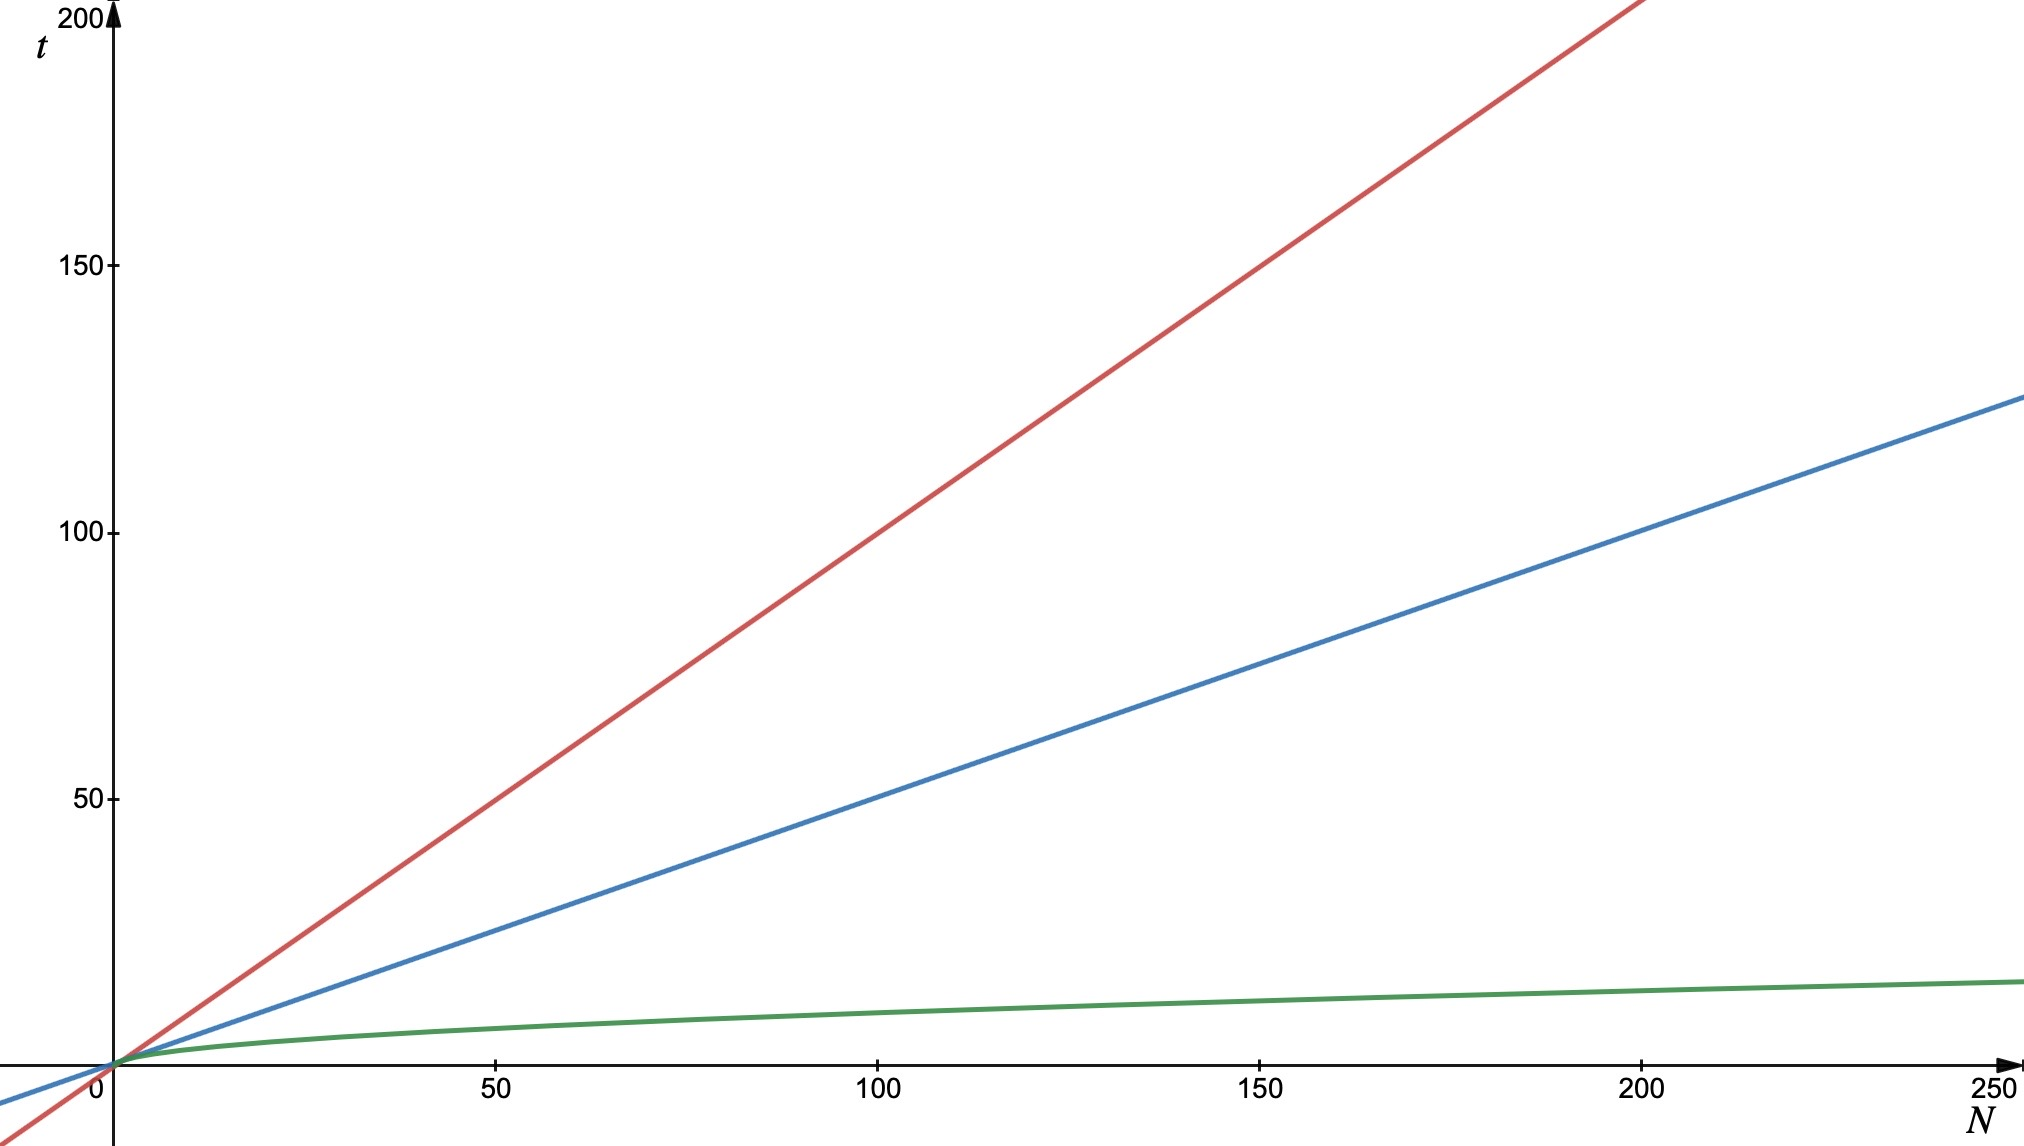
\includegraphics[width=0.7\textwidth]{figures/laufzeit-aufgabenstellung.jpg}
    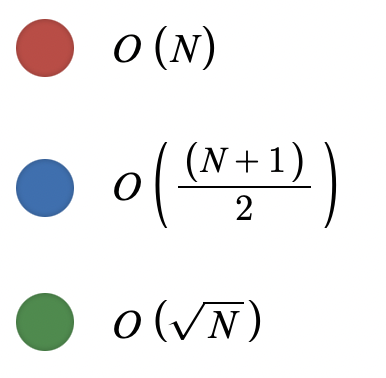
\includegraphics[width=0.165\textwidth]{figures/legende.png}

    \caption{Schlechteste (rot) und durchschnittliche (blau) erwartete Laufzeit einer Suche bei einem 
    \\klassischen Rechner sowie die Laufzeit des Grover Algorithmus (grün) 
    \\Quelle: Eigene Darstellung}

	\label{fig:laufzeitAufgabenstellung}
\end{figure}

\section{Grovers-Algorithmus $\mathbf{\textsubscript{\small tp}}$}
Um den Algorithmus besser verstehen zu können, werden die Rahmenbedingungen formalisiert. Die Datenbank, besitzt $\mathbf{N}$ Elemente wobei  $\mathbf{N = 2^n}$ entspricht. Den Datensätzen ordnen wir die Elemente $\mathbf{ \{ 0,1 \}^n}$ zu. Wenn $\mathbf{ n=2}$ entspräche erhielt man die Elemente $\mathbf{00,01,10,11}$. Das gesuchte Elemente bezeichnen wir als  $\mathbf{\hat{x}}$. Die Datenbank wird als eine Funktion $\mathbf{f \{ 0,1 \}^n  \rightarrow \{ 0,1 \}}$ mit folgender Eigenschaft umgesetzt: \\
$\mathbf{f(x) = \begin{cases}1 \quad f\ddot{u}r \,
		x = \hat x \\0 \quad sonst \end{cases} 
}$ 
\newline
Mithilfe dieser Funktion haben wir unser Quantenorakel. $\mathbf{U_f : | x,y \rangle \to |x,y \oplus f(x) \rangle}$. Die Funktion $\mathbf{f}$gibt nur ein zurück, wenn die Eingabe das gesuchte Element $\mathbf{\hat x}$ ist. Das Quantenorakel, negiert daher nur das Vorzeichen des gesuchten Elements. 

\subsection{Prinzip}
Der Grover Algrothmus lässt sich in drei Schritte aufteilen.
\begin{enumerate}
	\item \textbf{Superpositionen aufbauen}
	\\
	im ersten Schritt werden alle Quantenbits in die Superposition gebracht.
	\item \textbf{Amplitudenveränderung durchführen} \emph{(Grover Iteration G)}
	\\
	Der Zweite Schritt verändert die Amplituden der Elemente. Dabei wird die Amplitude des gesuchten Elementes erhöht und alle anderen verringert. Dieser Schritt wird auch \emph{(Grover Iteration G)} genannt und abhängig von der Anzahl der Elementen öfters wiederholt. Wie oft die Grover Iteration ausgeführt werden muss, wird im Abschnitt \ref{sec:geoVer} erläutert.
	\item \textbf{Messen} 
	\\
	Im letzten Schritt werden die Quantenbits gemessen und man erhält mit einer hohen Wahrscheinlichkeit, das gesuchte Element $\mathbf{\hat x}$.
\end{enumerate}

\subsubsection{Amplitudenveränderung}
Die Amplitudenveränderung besteht aus zwei Schritten. Beim ersten Schritt handelt es sich um die Negation der Amplitude von $\mathbf{\hat x}$. Im zweiten Schritt wird die negative Amplitude ausgenutzt um die Amplitude zu verstärken. Dies passiert in dem alle Amplituden am Mittelwert aller Amplituden gespiegelt werden. 
\\ \\
\textbf{Negieren der Amplitude}
 \\
Um die Amplitude von $\mathbf{\hat x}$ zu negieren, wird ein Hilfsbit benötigt. Das Hilfsbit wird in den Zustand $\mathbf{H|1\rangle}$ mithilfe eines Hadamar Gatters gebracht. Dadurch erhalten wird $\mathbf{|x\rangle \frac{1}{\sqrt 2}(|0\rangle - |1\rangle )}$. Anschließend wird das Quantenorakel angewendet und damit das Vorzeichen der Amplitude des gesuchten Elementes negiert. Das Hilfsbit wird nun nicht mehr benötigt und kann in folgenden Berechnungen weggelassen werden. Dies lässt sich auch an folgender Abbildung erkennen. Dort ist Anwendung des Quantenorakel und beispielhaft die Amplituden alle Elemente der Datenbank vor und nach der Anwendung des Quantenorakels zu sehen.
\begin{figure}[hbtp]
	\centering
	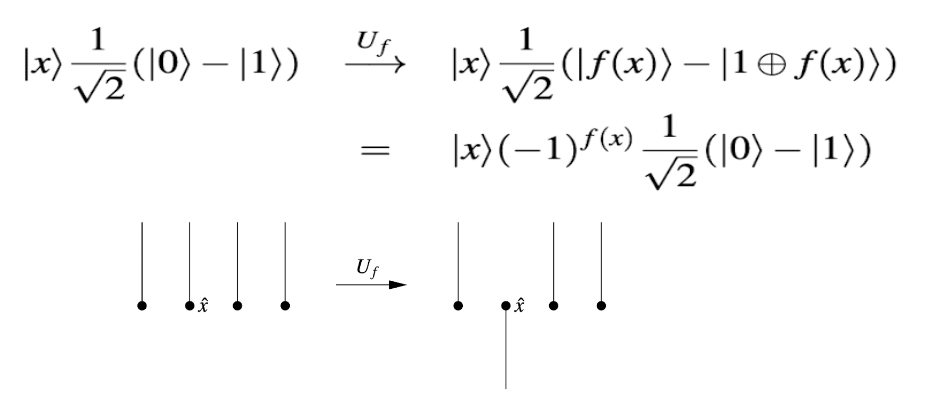
\includegraphics[width=.8\textwidth]{figures/amplitudenveraenderung.png}
	\caption{Amplitudenveränderung}
	\label{fig:changeAmplitude}
\end{figure}
Die negative Amplitude von $\mathbf{\hat x}$ hat keinen Einfluss auf das Messen, um mit einer erhöhten Wahrscheinlichkeit das Element $\mathbf{\hat x}$ nach dem Messen zu erhalten benötigt man den Schritt Spiegeln am Mittelwert.
\\\\
\textbf{Spiegelung am Mittelwert} \\
\label{sec:spiegelnAmMittelwert}
Um zu zeigen, das die Spiegelung der Amplituden am Mittelwert den gewünschten Effekt hat, folgen nun einige Beispiel Rechnungen. Eine Spiegelung an einem wert $\mathbf{m}$ entspricht der Abbildung: $\mathbf{\alpha \rightarrow 2 \times m - \alpha}$. \\
Nimmt man an die Datenbank enthält vier Elemente ($\mathbf{n=2}$) so entspricht - nach der Negation von $\mathbf{\hat x}$ - der Mittelwert $\mathbf{m = \frac{1}{4} \times (\frac{1}{2}- \frac{1}{2}+ \frac{1}{2} +\frac{1}{2}) = \frac{1}{4}}$. Die Spiegelung von $\mathbf{\hat x}$ entspricht $\mathbf{-\frac{1}{2} \times \frac{1}{4} - (-\frac{1}{2}) = 1}$. Damit ist die Amplitude des gesuchten Elements gleich eins. Würde man nun die Bits messen, erhält man mit einer Wahrscheinlichkeit von 100\% das Element $\mathbf{\hat x}$. Die Amplituden aller anderen Elemente entwickeln sich wie folgt: $\mathbf{\frac{1}{2} \times \frac{1}{4} - \frac{1}{2} = 0}$
\\ \\
Wäre $\mathbf{n = 3}$, so würde die Amplitude von $\mathbf{ \hat x}$ nach der ersten Grover Iteration $\mathbf{\frac{5}{5\sqrt 8}}$ und alle anderen Amplituden $\mathbf{\frac{1}{2\sqrt 8}}$ betragen. Nach einer Spiegelung am Mittelwert ist die Amplituden von $\mathbf{\hat x}$wieder positiv, bevor ein erneutes Spiegeln möglich ist um die Amplitiduen weiter zu verstärken oder zu verringern, muss zuerst erneut das Quantenorakel angewandt werden. Ein erneutes Spiegeln, nach der Negation, der Amplituden würde diese wie folgt verändern. Das gesuchte Element $\mathbf{\hat x}$ hätte eine Amplitude von $\mathbf{0,973}$, alle anderen Elemente eine von $\mathbf{-0, 088}$. Würde nun gemessen werden erhielte man mit einer Wahrscheinlichkeit von 93 \% das gesuchte Element.
\\ Ein erneutes Spiegeln würde die Amplituden des gesuchten Elementes  im Gegensatz zu Erwartung wieder verringern und alle anderen erhöhen, daher ist es besonders wichtig, dass nicht zu viele Grover Iterationen ausgeführt werden. Wie die Genaue Anzahl an Iterationen jedoch berechnet werden kann, folgt im Abschnitt \ref{sec:geoVer}
\textbf{SOUFFLE?}
\subsubsection{Graphische Darstellung des Grover Algorithmus}
Der Grover Algorithmus sieht nach dem bisherigen Erklärungen wie folgt aus.
\begin{figure}[hbtp]
	\centering
	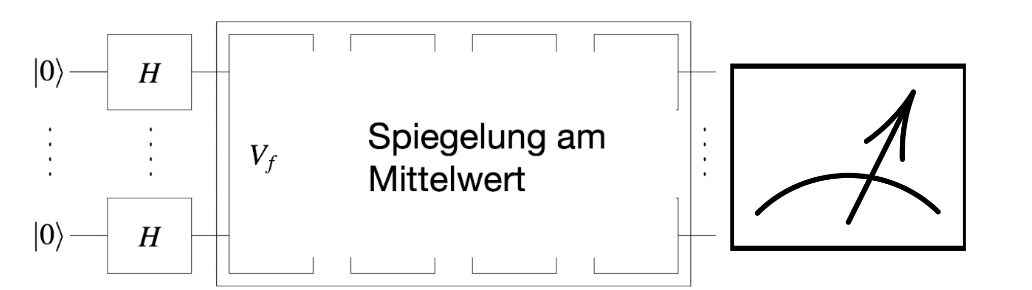
\includegraphics[width=1\textwidth]{figures/algotInformell.png}
	\caption{Graphische Darstellung des Grover Algorithmus \\ Quelle EIGENS ERSTELLEN!!!! }
	\label{fig:algotInformellt}
\end{figure}
Alle Bits werden mithilfe der Hadamar Gatter in Superpositionen gebacht. Alles danach bis zum Messen Symbol am Ende ist die Grover Iteration.
Der Äußere Kasten steht für das mehrfache Wiederholen dieser Iterationen. $\mathbf{V_f}$ steht für das Quantenorakel, jedoch wird hier das Hilfsbit nicht mit eingezeichnet.  Anschließend folgt die Spiegelung am Mittelt, wie diese genau mithilfe von Gattern umgesetzt wird folgt im nächsten Abschnitt \ref{sec:realiserung}. Nach dem ausführen der Grover Iterationen werden die Bits gemessen.
\subsection{Realisierung der Spiegelung am Mittelwert}
\label{sec:realiserung}
Die Abbildung $\mathbf{\alpha \rightarrow 2 \times m - \alpha}$ lässt sich mithilfe einer Matrixberechnung umsetzten.
\begin{center}
	$\mathbf{D_N \times 
	\begin{pmatrix}
			\alpha_0 & \alpha_1 & \dots &\alpha_{N-1}
	\end{pmatrix}^T, \text{mit } D_N = 
	\begin{pmatrix}
			-1 + \frac{2}{N} & \frac{2}{N} & \dots& \frac{2}{N} \\
			\frac{2}{N} & -1 \frac{2}{N} & \dots& \frac{2}{N} \\
			\vdots & \vdots & \ddots& \dots \\
			 \frac{2}{N} & \frac{2}{N} & \dots& -1+ \frac{2}{N} \\
	\end{pmatrix}}$
\end{center}
\subsubsection{Beispielrechnung}
Sei $\mathbf{N = 4}$ so ergibt sich folgende Rechnung:
\begin{center}
 $\mathbf{D_4  \times \begin{pmatrix}
		0,5 & -0,5 & 0,5 & 0,5
\end{pmatrix}^T}$.

$\mathbf{\begin{pmatrix}
		-0,5 & 0,5 &0,5&0,5\\
		0,5 & -0,5 &0,5&0,5\\
		0,5 & 0,5 &-0,5&0,5\\
		0,5 & 0,5 &0,5&-0,5
	\end{pmatrix}
	\times \begin{pmatrix} 0,5 \\ -0,5 \\ 0,5 \\ 0,5 \end{pmatrix} = \begin{pmatrix} 0\\1\\0\\0 \end{pmatrix}
}$.
\end{center}
Dieses Ergebnis gleicht sich mit dem Ergebnis aus Abschnitt \ref{sec:spiegelnAmMittelwert}, in dem wir ebenfalls alle Elemente einer Datenbank mit $\mathbf{N=4}$ Elementen an dem Mittelwert der Amplituden gespiegelt haben. Folgende Abbildung zeigt ebenfalls nochmal wie sich die Amplituden verändert haben.
\begin{figure}[hbtp]
	\centering
	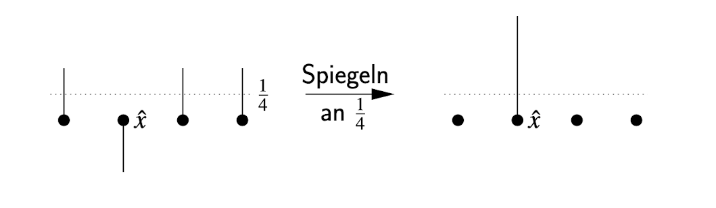
\includegraphics[width=.8\textwidth]{figures/spiegelung.png}
	\caption{Spiegelung am Mittelwert \\ Quelle: HOEMEISTER SEITE}
	\label{fig:spiegelung}
\end{figure}
Wenn eine $\mathbf{N \times N}$ Matrix verwendet wird, dann verstößt dies gegen das Lokalitätsprinzip. Daher muss die $\mathbf{D_n}$ Matrix in verschiedene unitäre Matrizen zerlegt werden.  $\mathbf{D_n}$ kann in ein Produkt aus drei unitäre Matrizen zerlegt werden.
\begin{center}
$\mathbf{D_n = -H_n \times R_N \times H_n, \text{mit } R  = 
\begin{pmatrix}
		-1 & 0 &\dots& 0 \\
		0& 1& \ddots& \vdots\\
		\vdots &\ddots& \ddots&0 \\
		0& \dots& 0 &1 \\
\end{pmatrix}}$
\end{center}
\subsubsection{Beispielrechnung}
Um zu zeigen, das die Matrix $\mathbf{D_N}$ wie oben als Produkt dreier Matrizen zerlegt werden kann, folgt ein Beispiel mit $\mathbf{D_4}$.
\begin{figure}[hbtp]
	\centering
	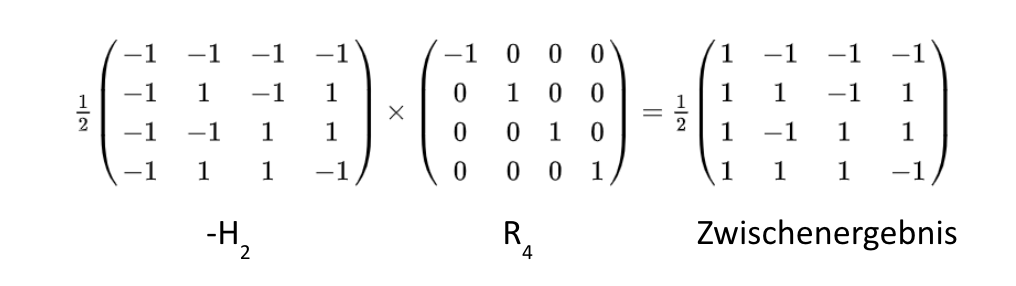
\includegraphics[width=.8\textwidth]{figures/householderLokal_1.png}
	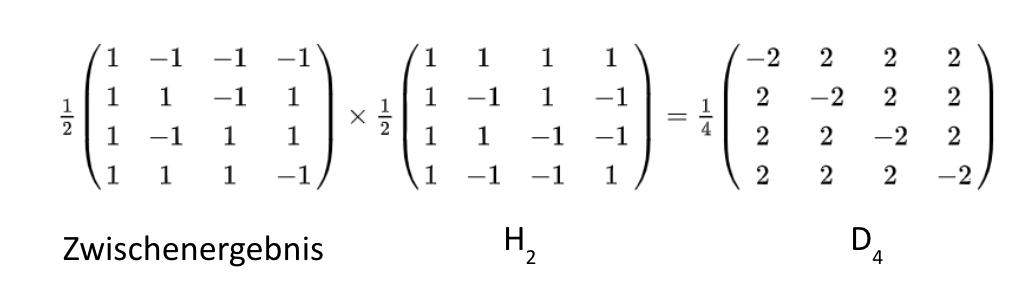
\includegraphics[width=.8\textwidth]{figures/householderLokal_2.png}
	\caption{Beispielzerlegung von $\mathbf{D_4}$ \\ Quelle: eigene Darstellung}
	\label{fig:DLokal}
\end{figure}
Das Ergebnis der Berechnung ist wie in der beschriftetet Rechnung \ref{fig:DLokal}) zu sehen gleich mit der zu erwarteten Matrix $\mathbf{D_4}$. Der Beweis, das dies auch für beliebige $\mathbf{N}$ zutrifft befindet sich in dem Buch vom Hoemeister auf der Seite 309 QUELLE.

\subsubsection{Matrix R als lokale Transformation}
Es wurde gezeigt, das die Matrix $\mathbf{D_N}$ in ein Produkt aus Matrizen zerlegt werden kann. Das die Hadamar Matrixen mit Hilfe eines Gattern als lokale Transformation umgesetzt werden können ist bekannt. Dies muss jedoch auch noch für $\mathbf{R_N}$ gezeigt werden. 
\\
Um ein Gatter zu entwickeln zu können, welches die Transformation $\mathbf{R_N}$ umsetzt, muss sich angeschaut werden wie sich $\mathbf{R_N}$ bei einer Multiplikation von Matrizen auswirkt. Alle Werte einer Matrix die mit $\mathbf{R_N}$ multipliziert wird bleiben gleich. Lediglich die erste Zeile oder Spalte wird negiert. Dies ist davon abhängig, ob die Matrix $\mathbf{R_N}$ auf der Linken oder Rechten Seite der Multiplikation ist. In ersten Zeile der Abbildung \ref{fig:DLokal} ist die Negation der ersten Spalte zu sehen.
\\
Multipliziert man $\mathbf{R_N}$ mit Amplituden, bedeutet dies, dass lediglich die Amplitude des ersten Elementes ($\mathbf{|0...0\rangle}$)negiert wird.
Falls $\mathbf{R_4}$ wäre, dann sähe das Gatter wie in Abbildung \ref{fig:Rgatter} aus.
 \begin{figure}[hbtp]
 	\centering
 	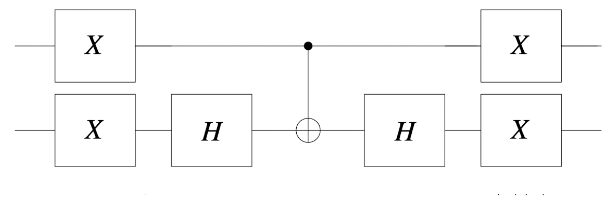
\includegraphics[width=.8\textwidth]{figures/rgatter.png}
 	\caption{$\mathbf{R_4}$ Realisierung \\ Quelle: HOEMEISTER SEITE}
 	\label{fig:Rgatter}
 \end{figure}
\\
Es folgt eine weitere Beispielrechnung, um zu verdeutlichen, das dieses Gatter die Transformation $\mathbf{R_4}$ ausführt.
\subsubsection{Beispielrechnung}
ABBILDUNG
 In den Abbildungen () werden die Werte der QBits $\mathbf{|00\rangle}$ und wie diese sich durch die einzelnen Gatter verändern dargestellt.
 Die Pauli X Gatter invertieren den Wert eines QBits. Aus $\mathbf{|0\rangle}$ wird $\mathbf{|1\rangle}$ und andersrum. Das erste Bit wird bis zum letzten Pauli-X Gatter nicht mehr verändert. Es wird ausschließlich genutzt um zu schauen, ob das CNOT aktiviert wird. Das zweite QBit wird durch das erste Hadamar Gatter, in folgende Superposition $\mathbf{\frac{1}{\sqrt 2}(|0\rangle - |1\rangle)}$. Da das erste QBit den Wert $\mathbf{|1\rangle}$ hat wird das zweite QBit durch das CNOT negiert - $\mathbf{-\frac{1}{\sqrt 2}(|0\rangle - |1\rangle)}$. Anschließend durch läuft das zweite Bit wieder ein Hadamar Gatter, das QBit hat anschließend folgenden Wert: $\mathbf{-|1\rangle}$.
 Zum Schluss werden beide Bits ($\mathbf{|1\rangle}$ und $\mathbf{-|1\rangle}$) durch die Pauli-X Gatter invertiert und wir erhalten das gewünschte Ergebnis von $\mathbf{-|00\rangle}$.
  \\
  \\
  ABBILDUNG

 Die Abbildung () zeigt die QBits $\mathbf{|01\rangle}$  und wie diese von den Gattern verändert werden. Die ersten Pauli-X Gatter invertieren abermals die QBits, diese haben nun den Wert $\mathbf{|10\rangle}$. Das erste QBit wird bis auf von dem letzten Pauli-X Gatter nicht verändert und nur zur Aktivierung der Operation CNOT zuhilfe genommen. Das zweite QBit wird durch das Hadamar Gatter in die Superpostion $\mathbf{\frac{1}{\sqrt 2}(|0\rangle + |1\rangle)}$ gebracht. Diese verändert sich auch nicht durch die CNOT Operation. Nach der CNOT Operation wird das QBit durch das zweite Hadamar Gatter wieder in den Basiszustand $\mathbf{|0\rangle}$ gebracht. Zuletzt durchlaufen die beiden QBits ein Pauli-X Gatter welches die QBits von den Basiszustände $\mathbf{|10\rangle}$ in den erwarteten Zustand $\mathbf{|01\rangle}$ überführt. Die QBits haben nach dem durchlaufen des Gatters die selben Zustände wie vorher.
  \\ 
  \\
Bei den QBits $\mathbf{|10\rangle \text{ und }|11\rangle}$, wird die CNOT Operation nicht ausgeführt, da das erste QBit in den Basiszustand $\mathbf{|0\rangle}$ überführt werden. Die QBits werden durch die doppelte Ausführung der Gatter ebenfalls nicht verändert.
\\
\\
Daran kann gesehen werden, dass die Gatter die gewünschte Operation $\mathbf{R_4}$ ausführen.

\subsection{Graphische Darstellung des Grover Algorithmus}
In der Abbildung() ist wie in der Abbildung() der Grover Algorithmus nochmals Graphisch dargestellt. Dieses mal enthält die Abbildung alle verschiedenen Gatter, die die QBits durchlaufen.





\section{Bestimmung der Anzahl an Grover-Iterationen $\mathbf{\textsubscript{\small tp}}$}
Nachdem der genaue Ablauf des Algorithmus erklärt wurde, bleibt die Frage: Wie oft muss die Grover Iteration durchgeführt werden, um mit einer hohen Wahrscheinlichkeit das gesuchte Element $\mathbf{\hat{x}}$ zu messen? noch offen.

\subsection{Geometrische Veranschaulichung}
Mithilfe von Regeln aus der Geometrie kann die Anzahl der Iterationen bestimmt werden. Das Schrittweise erhöhen der Amplitude des gesuchten Elements kann auf der Bloch Kugel als Rotation aufgefasst werden. 
\\
In der Geometrie entspricht die Spiegelung eines Punktes an zwei Ebenen eine Drehung um den Winkel $\mathbf{2 \times \beta}$, wobei $\mathbf{\beta}$ der Winkel zwischen den Ebenen ist. Dies ist in der Abbildung \ref{fig:zweiEbenen} verdeutlicht. Diese Eigenschaft kann sich zunutze gemacht werden. Ist der Winkel bekannt, kann ausrechnet werden, um wie viel der Grad gedreht werden muss, um das gesuchte Element zu erreichen und damit wie oft die Grover-Iteration durchgeführt werden muss.
 \begin{figure}[hbtp]
	\centering
	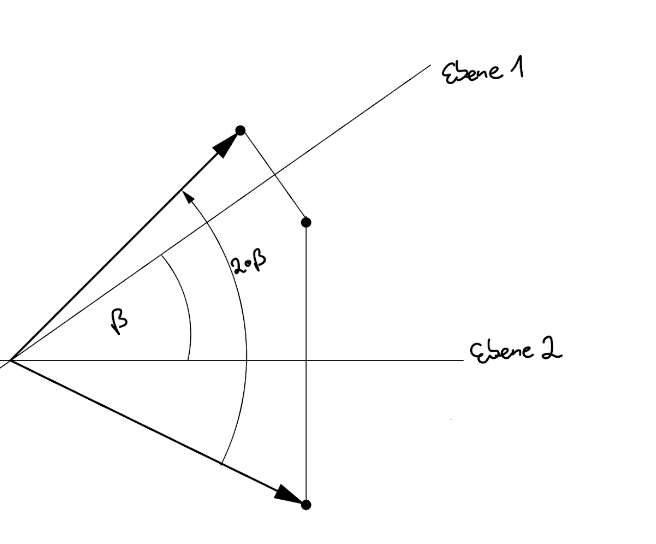
\includegraphics[width=.6\textwidth]{figures/zweiEbenen.png}
	\caption{$\mathbf{R_4}$ Spiegelung an zwei Ebenen \\ Quelle: Anlehnung an \cite[S. 149]{Ho17}}
	\label{fig:zweiEbenen}
\end{figure} 
\noindent
\\
Wie der Name schon sagt, handelt es sich bei der Spiegelung am Mittelwert um eine Spiegelung. Die zweite Spiegelung ist das negieren von dem gesuchten Element $\mathbf{\hat{x}}$. Die Formel zur Spiegelung an einem Wert $\mathbf{m}$ lautet: $\mathbf{\alpha \rightarrow 2 \times m - \alpha}$. Ist $\mathbf{m=0}$ erhalten wir $\mathbf{\alpha \rightarrow - \alpha}$. Dies zeigt, dass die Negation eines Elementes eine Spiegelung an dem Wert $\mathbf{0}$ ist.
\\ 
\\
Der Winkel lautet $\mathbf{\sin(\beta) = \langle s | \hat{x} \rangle}$, mit $\mathbf{s = \frac{1}{\sqrt{N}}\sum\limits_{x=0}^{N-1}|x\rangle}$, welches die Allgemeine Superposition ist. Ausrechnet ergibt dies $\mathbf{\sin(\beta) = \frac{1}{\sqrt N}}$. Daran lässt sich erkennen, dass die Anzahl der Iterationen abhängig von der Anzahl der Datenbankelemente ist und nicht von $\mathbf{\hat{x}}$. Wäre dies nicht so, hätte das zur Folge, dass für jedes gesuchte Element die Anzahl der Grover Iterationen angepasst werden müsste.
\subsubsection{Beispielrechnung: Geometrische Veranschaulichung}
Sei $\mathbf{N=4}$, dann folgt daraus, dass $\mathbf{\sin(\beta) = \frac{1}{\sqrt{4}}}$ ist. Nach Beta aufgelöst ergibt sich $\mathbf{\beta = \frac{\pi}{6}}$.
\\
Wird nun eine Grover Iteration durchgeführt, ändert sich der Winkel wie folgt: $\mathbf{\beta = \frac{\pi}{6} + 2 \times \frac{\pi}{6}  = \frac{\pi}{2}}$. Wird nun $\mathbf{sin(\frac{\pi}{2}))}$ ausgerechnet, erhalten wir $\mathbf{1}$. Dies bedeutet, dass wir mit einer Drehung das gesuchte Element erreicht haben. Wird nun gemessen, erhalten wir mit einer Wahrscheinlichkeit von 100 \% das gesuchte Element. Dies wird auch wie im Abschnitt  \ref{sec:spiegelnAmMittelwert}  beschrieben erwartet.

\subsubsection{Anzahl an Grover Iterationen}
Durch die Rechnung konnte gezeigt werden, dass der Startwinkel $\mathbf{\frac{1}{\sqrt{N}}}$ beträgt und der Winkel nach $\mathbf{T}$ Grover Iterationen der Winkel den Wert $\mathbf{(2 \times T + 1)\times \frac{1}{\sqrt{N}}}$ hat. 
Falls für $\mathbf{T = \frac{\pi}{4}\times \sqrt{N}}$ gewählt wird, wird immer sehr nah an das gesuchte Element rotiert. 
\\
In der praktischen Umsetzung muss $\mathbf{T}$ immer abgerundet werden, da nur eine gerade Zahl an Iterationen durchgeführt werden kann. Wird $\mathbf{T}$ aufgerundet, werden zu viele Grover-Iterationen durchgeführt und es wird sich vom gesuchten Element wieder entfernt. \cite[S. 157]{KLM07} Das Souffl\'{e} würde anfangen einzugehen
\\
\\
Dadurch, dass die Anzahl der Grover-Iterationen $\mathbf{ \frac{\pi}{4}\times \sqrt{N}}$ beträgt und in jeder Iteration einmal das Quantenorakel aufgerufen wird, beträgt die Laufzeit des Grover Algorithmus $\mathbf{O(\sqrt N)}$.

\label{sec:geoVer}

\section{Varianten der Quantensuche $\mathbf{\textsubscript{\small sc}}$}
Grovers Suchalgorithmus lässt sich so anpassen, dass er auch auf ähnliche verwandte Probleme angewandt werden kann. Bisher wurde für den Algorithmus vorausgesetzt, dass f genau ein Element xDACH auf 1 abbildet und die anderen Elemente auf 0. Diese Voraussetzung ist aber nicht bei jeder Suche gegeben. In den folgenden Abschnitten werden Suchalgorithmen betrachtet, bei denen es mehr als eine korrekte Lösung und unbekannt viele Lösungen gibt. Abschließend wird in Abschnitt x die Suche nach dem Minimum betrachtet. 

\subsection{Suche nach einer von mehreren Lösungen}

Angenommen in der Menge der möglichen Lösungen N befindet sich nicht nur ein Element xDACH, welches f auf 1 abbildet, sondern mehrere. Bei der Suche mit einem klassischen Computer verringert sich die Anzahl der Auswertungen von f\(x\) entsprechend der Anzahl der vorhandenen Lösungen. So würde bei vier korrekten Lösungen in N nur noch ein Viertel der ursprünglichen Auswertungen zu erwarten sein.
Auch bei der Quantensuche verringert sich der Aufwand entsprechend, ohne eine große Modifizierung am Algorithmus vorzunehmen.
Für die Suche nach einer von mehreren Lösungen ist wieder ein Orakel UVONf gegeben, wobei die Funktion f genau k Elemente xDACH1, … xDACHk auf 1 abbildet. k ist somit die bekannte Anzahl der Lösungen in N, mit N \\= 2\^n. Der Algorithmus besteht wieder aus den folgenden Schritten\:

1. Es wird die gleichverteilte Superposition aufgebaut, indem alle Qubits in die Superposition gebracht werden:
R ← Hn 0…0  
2. Grover-Iteration auf R anwenden und so die Amplitudenveränderungen durchführen. 
R ← -HnENHnVf x
Die Grover-Iteration wird dabei G\(N,k\)-mal ausgeführt
3. Das Quantenregister R wird gemessen und die Ergebnisse ausgegeben.

Der einzige Punkt, in dem sich dieser Algorithmus von dem ursprünglichen Grover-Algorithmus unterscheidet, ist im zweiten Schritt die Anzahl der Grover-Iteration. Im Regelfall wird die Grover-Iteration T\= pi\/4 x sqrt\(N\) durchgeführt. G\(N,k\) ist jedoch definiert mit:
G\(N,k\) ~\= pi\/4 sqrt\(N\/k\)
Damit reduziert die Anzahl der vorhandenen Lösungen in N die Anzahl der benötigten Grover-Iterationen. Für den Fall, dass k \>= 3\/4 N kann ein zufälliges Element x aus N gewählt und f\(x\) ausgewertet werden. Mit einer 75 prozentigen Wahrscheinlichkeit wird f\(x\) zu 1 auswerten.
Laufzeit

\subsection{Suche nach unbekannt vielen Lösungen}
Eine größere Herausforderung stellt die Suche dar, wenn im Vorhinein nicht bekannt ist, wie viele Lösungen in der durchsuchten Menge N vorhanden sind. Bisher wurde die Anzahl der Lösungen benötigt, um die Anzahl der Grover-Iterationen zu bestimmen, damit durch die Amplitudenveränderung mit großer Wahrscheinlichkeit das gesuchte Element gefunden wird. Ist die Anzahl der richtigen Elemente vorher nicht bekannt, so muss die Anzahl der Iterationen auf eine andere Weise bestimmt werden. Dazu wurde der Grover-Algorithmus von Boyer, Brassard, Høyer und Tapp weiterentwickelt und wird dementsprechend als G-BBHT-Suche bezeichnet.
Wie bei der Suche nach einer von mehreren Lösungen ist ein Orakel Uf gegeben, mit der Funktion f, die genau k Elemente xDACH1, …, xDACHk auf 1 abbildet und die restlichen Elemente auf 0. N ist wieder gegeben durch N\=n\^2, allerdings ist dieses mal nicht bekannt wie groß k ist. Der angepasste Algorithmus läuft folgendermaßen ab\:
1. Ein zufälliges Element x wird aus N ausgewählt. Wenn f\(x\) zu 1 auswertet wurde erfolgreich eins der gesuchten Elemente gefunden und es kann an dieser Stelle gestoppt werden. Hintergrund ist, dass k \>= 3\/4 N sein könnte und in diesem Fall mit großer Wahrscheinlichkeit auch ohne Iterationen ein korrektes Ergebnis erreicht werden kann. Wertet f\(x\) zu 0 aus, dann wird im 2. Schritt fortgefahren.
2. Es wird ein zufälliger Wert r ausgewählt mit r Element aus 1, … , sqrt\(N\). Dieses r bestimmt die Anzahl der Iterationen in Schritt 4.
3. Es wird die gleichverteilte Superposition aufgebaut, indem alle Qubits in die Superposition gebracht werden:
R ← Hn 0…0
4. Die Grover-Iteration wird r-mal auf R angewandt und so die Amplitudenveränderungen durchgeführt:
R ← -HnRNHnVfR
5. Das Quantenregister R wird messen und f\(x\) für das ausgegebene Ergebnis x ausgewertet. Wertet f\(x\) zu 1 aus, so wurde eins der gesuchten Elemente gefunden und es kann an dieser Stelle gestoppt werden. Wertet f\(x\) zu 0 aus, so wird wieder beim 1. Schritt begonnen.

Aus der Veröffentlichung von Boyer, Brassard, Høyer und Tapp geht hervor, dass bei Anwendung dieses Algorithmus nach einem Durchlauf eine Lösung mit einer Wahrscheinlichkeit von 25\% gefunden wurde. Trotz der zufällig gewählten Anzahl von Iterationen beträgt die Laufzeit für diesen Algorithmus O.
Boyer, Brassard, HoMITSTRICHyer und Tapp beschreiben eine weitere Modifizierung des Algorithmus, die es erlaubt die Laufzeit auf O zu senken. 
Dazu wird vor Beginn des Algorithmus ein SIGMA element aus \{1,…, 4\/3\} gewählt und m\=1 initialisiert. Die Anzahl der Iterationen r wird dann im 2. Schritt nicht mehr aus \{1, …, sqrt\(N\)\} gewählt, sondern aus \{0, …, m\}. Wertet f\(x\) im 5. Schritt dann zu 0 aus, wird m mit dem Faktor SIGMA multipliziert, sodass bei dem nächsten Durchlauf des Algorithmus im 2. Schritt r aus \{0, …, SIGMAm\} gewählt wird. Im schlechtesten Fall wird so lange keine Lösung gefunden, dass SIGMA x m \> sqrt\(N\) gilt. Dann wird im 2. Schritt r wieder zufällig aus \{0,  …, sqrt\(N\)\} gewählt, bis der Algorithmus terminiert. \[QUELLE\]


\subsection{Suche nach dem Minimum}
Bei den bisherigen Suchen wurde nur eine lokale Eigenschaft der Elemente berücksichtigt: handelt es sich bei dem aktuellen Element um jenes, welches ich suche? Vollkommen unabhängig von den anderen Elementen, die sich in N befinden. Bei der Suche nach dem Minimum ist jedoch eine globale Eigenschaft ausschlaggebend: Ist dieses Element kleiner, als alle anderen Elemente aus dem Feld? 
Zur Lösung dieses Problems haben 1996 Dürr und Høyer basierend auf der G-BBHT-Suche weiter gearbeitet und den folgenden Algorithmus entwickelt: 

Gegeben ist ein Orakel U, welches auf ein Feld T\[0\], …, T\[N-1\] zugreift. Dieses dient als Eingabe des Algorithmus, während das kleinste Element aus diesem Feld die Ausgabe des Algorithmus darstellt. N ist wieder gegeben durch 2\^n. Für das Orakel werden zwei Quantenregister x\> und y\> der Länge n, sowie ein Hilfsbit h\> verwendet\:

U formel und f formel

1. Schrankenindex wählen
Zu Beginn wird ein Anfangswert j für den Schrankenindex zufällig aus 0 <\= j <\= N-1 ausgewählt. Dieser wird genutzt, um das Register y\> zu initialisieren: y\> <\- j\>

2. Nach Dürr und HoMITSTRICHyer werden die folgenden Schritte wiederholt, bis die Gesamtlaufzeit 22.5 Sqrt\[N\] + 1.4 Log\[2,N\]\^2 überschreitet \[QUELLE\]. Anschließend wird mit Schritt 2.3. fortgefahren\:
2.1. Es wird die gleichverteilte Superposition aufgebaut, indem alle Qubits in die Superposition gebracht werden:
x\> <\- Hn 0…0  
2.2. G-BBHT-Suche
Auf dem Register x\> wird mit dem Quantenorakel U die G-BBHT-Suche ausgeführt. So wird aus alles Elementen des Feldes eines zufällig ausgewählt, welches kleiner als der Schrankenindex T\[y\] ist.
2.3 Das Quantenregister x\> wird gemessen. Gilt für das daraus resultierende Ergebnis i T\[i\]<T\[y\], dann wird y\> ← i\>  gesetzt.
3. Abschließend wird das Register y\> gemessen und das ausgegebene Ergebnis ist das kleinste Element des Feldes.

Der Algorithmus ist auf den ersten Blick, insbesondere durch die Verwendung der G-BBHT-Suche, recht abstrakt. Abbildung x soll das Verständnis  durch eine vereinfachte, grafische Darstellung des Vorgehens vereinfachen. Mit einer Laufzeit von O findet dieser Algorithmus mit über 50 \% das minimale Element des Feldes.


\section{Anwendungen des Grovers Algorithmus}
Wie zuvor gezeigt wurde, erreicht der Grovers Suchalgorithmus eine quadratische Beschleunigung im Vergleich zu klassischen Suchalgorithmen in unstrukturierten Datenmengen. 
Gerade im Hinblick auf $\mathbf{NP}$-vollständige Probleme stellt sich jedoch die Frage, ob eine noch größere Beschleunigung erreicht werden kann. Der Idealfall wäre eine exponentielle Beschleunigung der Suche. 
Diese Beschleunigung ist jedoch mit dem Grovers-Algorithmus nicht erreichbar. 
Es ist bewiesen, dass Grovers optimal ist \cite[S. 161-166]{Ho17}. 
Diese Limitierung ist relevant, wenn die Anwendungsmöglichkeiten von Grover betrachtet werden.
\subsection{klassische Datenbanken}
Grundsätzlich kann der Grover-Algorithmus eingesetzt werden, um klassische Datenbanken zu durchsuchen. 
Dazu wird allerdings ein aufwendiges Adressierungssystem benötigt, um die Verbindung zwischen klassischer Datenbank und Quantenhardware herzustellen. 
Ob dies zukünftig ein praktikabler Einsatzort für Quantensuchen wird, ist abhängig von der Entwicklung der verfügbaren Quantenhardware und deren Preisentwicklung.
\subsection{NP-vollständige Probleme}
Weiterhin lässt sich der Grovers-Algorithmus grundsätzlich für jedes Problem aus $\mathbf{NP}$ anwenden. 
So kann beispielsweise für das Traveling Salesperson Problem mithilfe der G-BBHT-Suche aus Kapitel \ref{gbbht} in $\mathbf{O(\sqrt{N})}$ eine Rundreise gefunden werden, die kürzer ist als eine gegebene Rundreise $\mathbf{k}$. 
Mit der Suche nach dem Minimum aus Kapitel \ref{minimum} kann sogar die kürzeste Rundreise aus $\mathbf{N}$ gefunden werden.

\begin{figure}
	\centering
	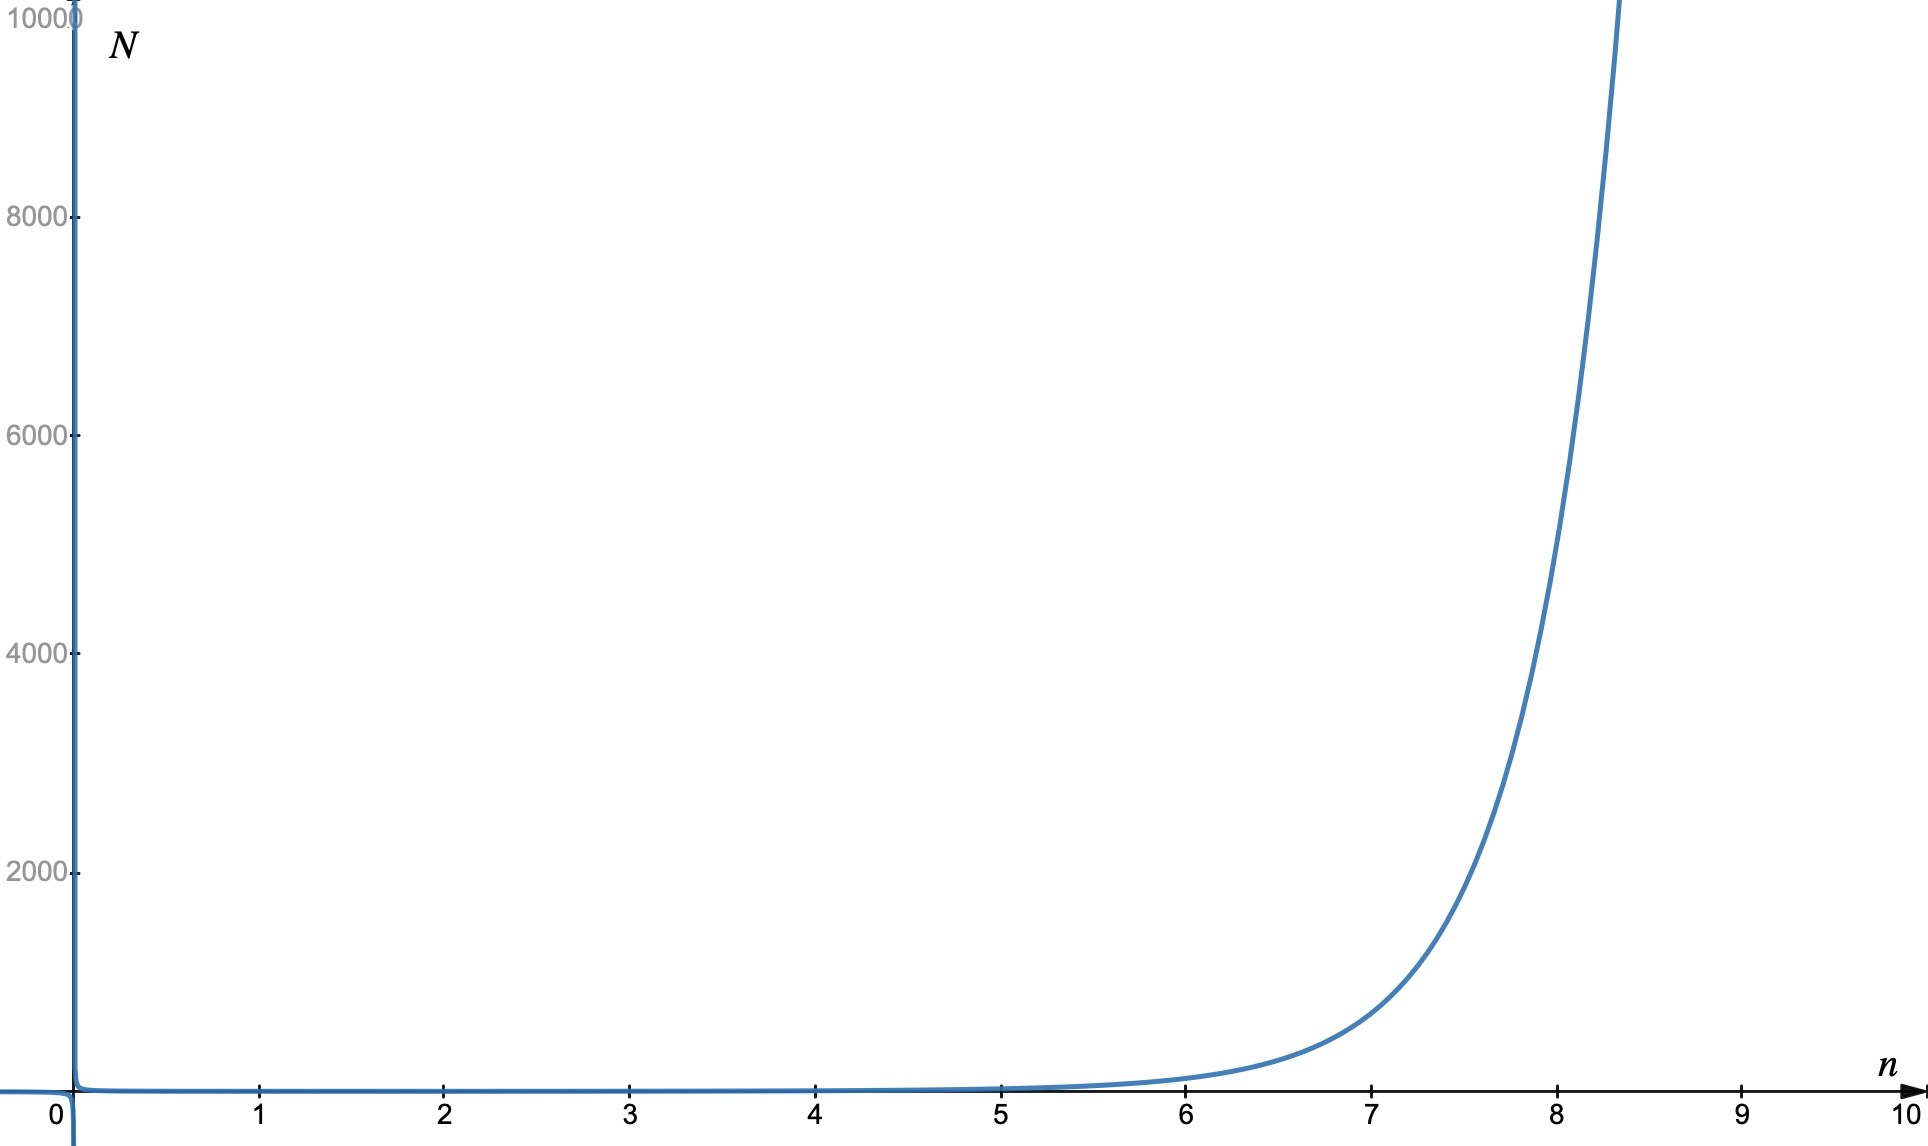
\includegraphics[width=0.7\textwidth]{figures/tsp.jpg}
	
	\caption{Exponentielles Wachstum der möglichen Rundreisen mit steigender Anzahl der Städte\\Quelle: Eigene Darstellung}
	
	\label{fig:tsp}
\end{figure}

In $\mathbf{N}$ liegt jedoch das limitierende Problem. Sollen beispielsweise $\mathbf{n}$ Städte besucht werden, so ergeben sich $\mathbf{N=(n-1)!}$ mögliche Rundreisen. 
\Cref{fig:tsp} zeigt, wie $\mathbf{N}$ im Verhältnis zu der Anzahl der Städte exponentiell wächst und somit verheerend groß wird. 
Die quadratische Beschleunigung durch den Grovers Algorithmus ist nicht ausreichend, um dieses Problem mit polynomialem Aufwand lösen zu können. 
Dazu wäre eine exponentielle Beschleunigung der Suche notwendig, dann könnte das Problem mit $\mathbf{\theta (n * \log n)}$ gelöst werden können. 
Da jedoch bewiesen ist, dass Grovers Algorithmus optimal ist, ist dies unmöglich.



\section{Folgen für die Fähigkeit von Quantencomputern }
Aus dem vorherigen Kapitel x ergibt sich, dass Grovers Algorithmus nicht ausreichend effizient ist, um alle NP-Probleme lösen zu können. Um alle Probleme aus NP lösen zu können, müssten für sehr verschiedene Probleme aus exponentiell großen Mengen von Lösungen die korrekten in polynomialer Laufzeit gefunden werden. Dies ist nur möglich, wenn all diese diversen Probleme eine gemeinsame Struktur aufweisen, welche auf die Fähigkeiten von Quantencomputern zugeschnitten und bisher nicht bekannt ist. Findet sich für ein Problem aus NP-vollständig ein effizienter Algorithmus, so ist davon auszugehen, dass ebenfalls diese gemeinsame Struktur erkannt wird und somit alle NP-vollständigen Probleme effizient lösbar werden.

\begin{comment}
\section{Verwendung}
Die GI gibt unter \url{http://www.gi-ev.de/LNI} Vorgaben für die Formatierung von Dokumenten in der LNI Reihe.
Für \LaTeX-Dokumente werden diese durch die Dokumentenklasse \texttt{lni} realisiert.

Dieses Dokument basiert auf der offiziellen Dokumentation, simplifiziert und setzt grundlegendes LaTeX-Wissen voraus.
Es werden generische Platzhalter an die entsprechenden Stellen (wie beispielsweise die Authoren-Angaben) gesetzt und nicht weiter an anderer Stelle dokumentiert.

Dieses Template ist wie folgt gegliedert:
\Cref{sec:demos} zeigt Demonstrationen der LNI-Verlage.
\Cref{sec:lniconformance} zeigt die Einhaltung der Richtlinien durch einfachen Text.

\section{Demonstrationen}
\label{sec:demos}
Das Symbol für Potenzmengen ($\powerset$) wird korrekt angezeigt.
Es ist kein Weierstraß-p ($\wp$) mehr.

Spitze Klammen können direkt eingegeben werden: <test />

Hier eine kleine Demonstration von \href{https://www.ctan.org/pkg/microtype}{microtype}:
\blindtext

\section{Demonstration der Einhaltung der Richtlinien}
\label{sec:lniconformance}

\subsection{Literaturverzeichnis}
Der letzte Abschnitt zeigt ein beispielhaftes Literaturverzeichnis für Bücher mit einem Autor \cite{Ez10} und zwei AutorInnen \cite{AB00}, einem Beitrag in Proceedings mit drei AutorInnen \cite{ABC01}, einem Beitrag in einem LNI Band mit mehr als drei AutorInnen \cite{Az09}, zwei Bücher mit den jeweils selben vier AutorInnen im selben Erscheinungsjahr \cite{Wa14} und \cite{Wa14b}, ein Journal \cite{Gl06}, eine Website \cite{GI19} bzw.\ anderweitige Literatur ohne konkrete AutorInnenschaft \cite{XX14}.
Es wird biblatex verwendet, da es UTF8 sauber unterstützt und \href{https://github.com/gi-ev/LNI/issues/5}{im Gegensatz zu lni.bst} keine Fehler beim bibtexen auftreten.

Referenzen sollten nicht direkt als Subjekt eingebunden werden, sondern immer nur durch Authorenanganben:
Beispiel: \Citet{AB00} geben ein Beispiel, aber auch \citet{Az09}.
Hinweis: Großes C bei \texttt{Citet}, wenn es am Satzanfang steht. Dies ist analog zu \texttt{Cref}.

Formatierung und Abkürzungen werden für die Referenzen \texttt{book}, \texttt{inbook}, \texttt{proceedings}, \texttt{inproceedings}, \texttt{article}, \texttt{online} und \texttt{misc} automatisch vorgenommen.
Mögliche Felder für Referenzen können der Beispieldatei \texttt{lni-paper-example-de.bib} entnommen werden.
Andere Referenzen sowie Felder müssen allenfalls nachträglich angepasst werden.

\subsection{Abbildungen}
\Cref{fig:demo} zeigt eine Abbildung.

\begin{figure}
  \centering
  \includegraphics[width=.8\textwidth]{example-image}
  \caption{Demographik}
  \label{fig:demo}
\end{figure}

\subsection{Tabellen}
\Cref{tab:demo} zeigt eine Tabelle.

\begin{table}
\centering
\begin{tabular}{lll}
\toprule
Überschriftsebenen & Beispiel & Schriftgröße und -art \\
\midrule
Titel (linksbündig) & Der Titel \ldots & 14 pt, Fett\\
Überschrift 1 & 1 Einleitung & 12 pt, Fett\\
Überschrift 2 & 2.1 Titel & 10 pt, Fett\\
\bottomrule
\end{tabular}
\caption{Die Überschriftsarten}
\label{tab:demo}
\end{table}

\subsection{Programmcode}
Die LNI-Formatvorlage verlangt die Einrückung von Listings vom linken Rand.
In der \texttt{lni}-Dokumentenklasse ist dies für die \texttt{verbatim}-Umgebung realisiert.

\begin{verbatim}
public class Hello {
    public static void main (String[] args) {
        System.out.println("Hello World!");
    }
}
\end{verbatim}

Alternativ kann auch die \texttt{lstlisting}-Umgebung verwendet werden.

\Cref{L1} zeigt uns ein Beispiel, das mit Hilfe der \texttt{lstlisting}-Umgebung realisiert ist.

\begin{lstlisting}[caption={Beschreibung}, label=L1, language=Java]
public class Hello {
    public static void main (String[] args) {
        System.out.println("Hello World!");
    }
}
\end{lstlisting}

\subsection{Formeln und Gleichungen}

Die korrekte Einrückung und Nummerierung für Formeln ist bei den Umgebungen
\texttt{equation} und \texttt{align} gewährleistet.

\begin{equation}
  1=4-3
\end{equation}
und
\begin{align}
  2&=7-5\\
  3&=2-1
\end{align}
\end{comment}
%% \bibliography{lni-paper-example-de.tex} ist hier nicht erlaubt: biblatex erwartet dies bei der Preambel
%% Starten Sie "biber paper", um eine Biliographie zu erzeugen.
\printbibliography

\end{document}
